\documentclass[12pt,a4paper]{book}
\usepackage[utf8]{inputenc}
\usepackage{amsmath}
\usepackage{amsfonts}
\usepackage{amssymb}
\usepackage{graphicx} % shows pictures
\usepackage{caption} % nice captions for figures
\usepackage{subcaption} % includes subfigure
\usepackage{nameref}
\usepackage{hyperref}
\usepackage{framed}
\usepackage{gensymb} % for \degree

\setcounter{secnumdepth}{3}

\title{Urge-Monitor\\Documentation}
\author{Christian Beck}
\begin{document}
\maketitle

\tableofcontents

\chapter{Basics}

\section{Runtime-Environment \& Dependencies}

The runtime environment of urge-monitor is setup with a provided script (\textit{setup-environment.sh} in the source root of this project). The runtime environment is a python virtual environment that contains all dependencies (on linux). To run the environment setup script you need a python3, python3-venv, pip3, gtk+3.0 (libgtk-3-dev) installed.

The runtime environment contains all dependencies needed to run urge-monitor - especially PsychoPy and all it's dependencies.

Urge-Monitor is developed with PsychoPy3, version 2020.1.2. Even though newer versions might work, using the exact version is recommended. Psychopy-packages for all platforms can be found at \url{https://github.com/psychopy/psychopy/releases} .

\paragraph{Note on versions:} It might be that the urge-monitor works fine with other versions of the above package (and it might even be that newer version improve on some qualities). However no other versions were extensively tested. No guarantee can be given for good performance or correct functioning if any other packages are used. The same argument applies also for single packages that Psychopy depends on.

\section{Installing the software}

Getting the software ready run is done in a few simple steps:

\begin{itemize}
	\item make sure everything is setup correctly
	\begin{itemize}
		\item[Linux] you need python3, python3-venv, pip3, gtk+3.0 (libgtk-3-dev)
		\item[Windows] you just need to install psychopy3 from the provided ressources and \dots
		\item[Mac] not tested, feel free to experiment
	\end{itemize}
	\item get the full package from github (\url{https://github.com/LueBecko/urge_monitor/})
	\item extract all files into a folder and go in that folder
	\item on Linux: run \textit{./setup-environment.sh}
\end{itemize}

Everything should be ready now to execute the software.

\section{Starting the software}

Before starting an experiment it is \textbf{strongly recommended} to close all other programs not necessary at runtime. Other programs that hog a lot of memory (like browsers), that can intercept other programs (like messengers) or can perform other costly actions on their own (like auto-updaters, storage and cloud programs, email-programs, server-applications \dots) should be closed to ensure as little as possible inference at runtime - good for low latencies in recording the urge and to avoid problems in displaying the stimuli.

Depending on which operating system is used the startup sequence varies.

\paragraph{Linux/Ubuntu}

Start the virtual environment of the experiment and run the file \emph{RunExperiment.py} in python.

\begin{verbatim}
	source .venv/bin/activate
	python3 urge_monitor/RunExperiment.py
\end{verbatim}

A shell script \emph{run.sh} containing all neccessary steps is present in the root directory of the software.

\begin{verbatim}
sh run.sh
\end{verbatim}

\paragraph{Windows}

This assumes that PsychoPy was installed with the downloaded installer package from GitHub - other methods might work in a similar fashion.

To start the software just invoke the python environment bundled with PsychoPy and run the \emph{RunExperiment.py} script. This has to be done from the console, e.g. 

\begin{verbatim}
C:\"Program Files (x86)"\PsychoPy3\python urge_monitor/RunExperiment.py
\end{verbatim}

This assumes that PsychoPy is installed at the above folder. Change the path if PsychoPy was installed on another path in your system.
A shell script \emph{run.bat} containing all neccessary steps is present in the root directory of the software.

\paragraph{MacOS}

During development no MacOS system was available. No information about how to install and run the software on MacOs can be given here. However PsychoPy does work on MacOS and with some effort one might be able to get the software running on MacOS.

\section{Users}

The design of the program incorporates two user classes: The experimenter and the subject. Both interact with the program in their unique non-overlapping modes.

However The controls for both users ae overlapping (mouse and keyboard control is present in both subject and experimenter). So both users are only independent by time (when they interact with the program), but not by channel. This means, that as soon as the experiment starts the experimenter should not touch the mouse or better disable (unplug?) his mouse/keyboard completely.

A third (artificial) actor in the experiment design is the MR-scanner, which serves as an external signal source, sending pulses for synchronization.

\section{Usage}

Figure \ref{fig:use} illustrates how the program is intended to be used.

\begin{figure}
	\includegraphics[width=\linewidth]{ressources/ExpUse1}
	\caption{Usage model of the program. The experimenter sets up an experiment, selects it to run at program startup, sets free parameters, start each run separately, which the subject performs and than exits the program.}
	\label{fig:use}
\end{figure}

The experimenter sets up the experiment. Then he runs it for each participant. He can select which experiment to run (in case several exist) when starting the program. Then he enters the (optional) free parameters for the subject. After that the program allows him to start the experiment runs - he can choose the order freely by clicking. By default the program goes through all runs in the given order. When a run is started the subject will see the bar and he can interact with it as intended. If fMRI-Simulation (\textit{pulse.ini}) is set to false, the program will start recording data after the first pulse, but is responsive from the beginning. After a run is finished the software gives control back to the experimenter.

%%%%%%%%%%%%%%%%%%%%%%%%%%%%%%%%%%%%%%%%%%%%%%%%%%%%%%%%%%%%%%%%%%%%%%%%%%%%%%%%
\chapter{Configurations}

Nearly every aspect of the application can be configured and adapted to suit any likely setting. Experiment and environment variables are given to the program in various \textit{.INI} files. Those INI-files need to be RFC 822 compatible, without support of interpolation (specific format strings for referencing within one INI-file). For the end-user this means: just write a valid value for each item and you won't have a problem.

\begin{center}
\begin{minipage}{0.85\linewidth}
\textbf{Syntax:}\\
\textbf{;} an comment, which will not be evaluated\\
\textbf{[}Section\_Name\textbf{]} \textbf{;} comment after section\\
Section\_Item1 \textbf{=} Value1\\
Section\_Item2 = Value2 \textbf{;} comment after item\\

\textbf{Value Syntax:} All INI-values get evaluated by python. So the written values should be python-readable.\\
\textit{Integer-value:} 0, 12, 1337, \dots \\
\textit{Float-Value:} 0.0, 1., 3.14, .455, \dots \\
\textit{Fields/Tuples:} (1, 2), [1024, 768], (0, -1, 1), \dots \\
\rule{2em}{0em} \textit{Colors:} (0, 255, 127), [255, 255, 0], \dots \\
\textit{Strings:} 'Hello World', 'Banana', \dots \\
\textit{Booleans:} True, False
\end{minipage}
\end{center}

A color is always a triple of numbers. The window section of the INI-file defines the used color space and therefore the possible values and meaning of each of those elements. This selection of a color space is binding for the whole project (even though the underlying framework allows to use different color spaces within one active window I decided against this usage for consistency and readability). (see section \ref{sec:color_spaces} \nameref{sec:color_spaces})

Read \emph{defaults.ini} to get an impression on the usage of those files, but be very careful if you want to change any parameter in this file, since this file is automatically loaded as reference on program start.

\section{Experiment Setup}

To run an experiment in the software the experimenter has to set up an experiment. This is done with a new subfolder in the folder \textit{exp} of the experiment source code. The name of the subfolder will be recognized as the name of the experiment. Within this folder the experimenter has to place a number of valid \textit{.INI} files.

\begin{itemize}
	\item \textbf{exp.ini} This file contains general information on how to setup the experiment.
	\item \textbf{input.ini} This file contains information about the used input device and how inputs are mapped to urge.
	\item \textbf{pulse.ini} This file describes how the software receives the start trigger pulse from the scanner.
	\item \textbf{monitor.ini} This file gives information about the hardware used to present the experiment and the target window.
	\item \textbf{defaults.ini} This file is optional. If it is not present in the folder of the experiment, it will be loaded from the root folder of the software. The file contains default information for visual stimuli and run control.
	\item \textbf{*.ini} A number of optional files corresponding to the runs of the experiment. Each run is defined by the values from \textit{defaults.ini}, but can be overwritten by their run-specific \textit{.ini} files.
\end{itemize}

When an experiment is loaded all files in its experiment definition folder will be read and validated. If any error is found in those files the program will stop.

\section{exp.ini}\label{sec:expini}

\textit{exp.ini} contains three sections: \verb|[main]|, \verb|[info]| and \verb|[runs]|. For an example of an experiment configuration see figure \ref{fig:expini}.

\verb|[main]| contains four items: \verb|[name]| (name of the experiment, string), \verb|log_folder| (path to write the log files, can be absolut or relative, string), \verb|abort_key| (defines the key to stop the running experiment at any time, key identifier), and \verb|log_buttons| (additional buttons which get logged, list of key identifiers, defautls to \verb|[]|)

\verb|[info]| can be empty. It contains fields which are used to annote the experiment runs of a single subject. Each entry in \verb|[info]| corresponds to one element in the experiment control GUI. If not present the entry \verb|subj| is added automatically (it is a string with the default subject name code). The field \verb|subj| is the only field in info which has an actual effect on program execution, since it goes into file- and folder-names as unique identifiers. All other entries get store into \textit{*.info} files and can be used for automatic reading of log-files. A string entry maps to a text-field which needs to be filed by the experimenter and is prefilled with the string value of the entry. A list maps to a single selection dropdown menu, where all entries of the list are given as options - the list entries should be string values.

\verb|[runs]| tells the the software how many runs are present, how are they named and if a dedicated configuration (aside from the \textit{defaults.ini}) should be applied to the run. Each entry in this section corresponds to a run. The order of runs is the order of entries. The name of an entry is the run name and will be presented in the experimenter GUI. The value of an run entry should be a string. If it is empty (\verb|''|) the run configuration is given by \textit{defaults.ini}. It can also contain the name of another \textit{.ini} file in the experiment setup folder. This file can contain any subset of entries from the \textit{defautls.ini} and overwrites those.

\begin{figure}
	\begin{framed}
		\begin{verbatim}
		[main]
		name = 'test_urge_fmri_exp'
		log_folder = 'logs'
		abort_key = 'q'
		log_buttons = ['y', 'x', 'c']
		
		[info]
		subj = 'Subject-Code'
		group = ['HC', 'GTS']
		
		[runs]
		run1 = 'run1.ini'
		run2 = 'run2.ini'
		run3 = ''
		\end{verbatim}
	\end{framed}
	
	\caption{Example \textit{exp.ini} file: sets up an experiment called \textit{test\_urge\_frmi\_exp}, stores log files in the folder \textit{logs} (relative to software root folder), can be aborted with the button \textit{q}, logs the buttons \textit{y}, \textit{x} and \textit{c}, asks for the subject code (\textit{subj}, defaults to \textit{Subject-Code}), asks for a group label (\textit{group}, either human control \textit{HC} or tourets \textit{GTS}), has three runs (named \textit{run1}, \textit{run2} and \textit{run3}, where the first and second load own configuration files and the third takes all its parameters from \textit{defaults.ini}). }
	\label{fig:expini}
\end{figure}

\section{input.ini}

This file only contains one section: \verb|[input]|. One entry is always present in this configuration file: \verb|device|. Its value is a string giving the name of the device interface which should be used to record responses in the experiment. \verb|device| can take one of the following values: \textit{Keyboard}, \textit{KeyboardHub}, \textit{MousePosAbs}, \textit{MousePosRel}, \textit{MouseWheel}, \textit{Auto}, \textit{Joystick}, \textit{JoystickAbs}.

\textit{Auto} is an device independent, automatic input generator, which is useful for testing and debugging purposes. It constantly moves the urge up and down (1 second for one move from max to min, min to max respectively).

\textit{Keyboard} and \textit{KeyboardHub} are interface to access the keyboard. \textit{Keyboard} is a low level fast interface, which only reacts to key press events (no way to act on continuous button presses). \textit{KeyboardHub} is a high level interface which reports all buttons currently pressed (including continuous button presses). Both interface need three additional entries for configuration: \verb|key_up|, \verb|key_down| and \verb|sensitivity|. \verb|key_up| and \verb|key_down| contain identifiers for keys that are pressed to either move the bar up or down. \verb|sensitivity| is a floating point number which gives the effect of a single button press ($0 \le urge \le 1, sensitivity = |\Delta urge|, 0 < sensitivity \le 1 $). (See figure \ref{fig:inputinikeyboard})

\textit{MousePosAbs} computes the urge value based on the absolute vertical position of the mouse pointer (which is hidden during experiment execution) on the screen (top of the screen translates to 1, bottom to 0). This interface works without further parameters. Sensitivity of this interface is based on the systems mouse sensitivity. 

\textit{MousePosRel} computes the urge value based on the relative vertical movement of the mouse. \verb|sensitivity| is a necessary parameter for this interface. It defines the translation between relative mouse movement and changes in reported urge. It needs to be set with much care - several tries might be necessary till a good value is found. (See figure \ref{fig:inputinimouse})

\textbf{NOTE:} \textit{MousePosAbs} has some problems on multi-monitor systems. In this case \textit{MousePosRel} should be used.

\begin{figure}
	\centering
	\begin{subfigure}[t]{0.4\linewidth}
		\begin{framed}
			\begin{verbatim}
			[input]
			device = 'MousePosRel'
			sensitivity = 0.5
			
			
			\end{verbatim}
		\end{framed}
		\caption{Use relative mouse position with a sensitivity of $0.5$.}
		\label{fig:inputinimouse}
	\end{subfigure}
	\quad
	\begin{subfigure}[t]{0.4\linewidth}
		\begin{framed}%[width = 0.4\linewidth]
			\begin{verbatim}
			[input]
			device = 'KeyboardHub'
			sensitivity = 0.05
			key_up = 'up'
			key_down = 'down'
			\end{verbatim}
		\end{framed}
		\caption{Use the keyboard (with io hub) with sensitivity of $0.05$. The up-arrow key increases the reported urge, the down-arrow key decreases the reported urge.}
		\label{fig:inputinikeyboard}
	\end{subfigure}
	
	\caption{Two example configurations of \textit{input.ini}}
	
\end{figure}

\textit{MouseWheel} allows update of the reported urge value through the vertical wheel of the mouse. \verb|sensitivity| is a necessary parameter for this interface. It defines the translation between wheel movement and changes in reported urge. It needs to be set with much care - several tries might be necessary till a good value is found.

\textit{Joystick} and \textit{JoystickAbs} are two unsupported interfaces. Because of incomplete support for devices, interfaces and operating systems the two device interfaces are not working correctly. It might be possible to develop working reliable interfaces, but this has no priority for the current project. Both incomplete joystick interfaces are part of the software, but should not be used, except for development.

\section{pulse.ini}

\textit{pulse.ini} contains all parameters regarding pulses send to external devices and received from external devices. It contains one section \verb|[pulse]|, which contains top level information on pulse configuration. It contains 
\begin{itemize}
	\item \verb|simulation| a boolean which indicates if pulse actually meassured - False - or generated artificially 2.5 sec after run start - True
	\item \verb|interface| a string defining the device interface for send and recieve pulses 
	\begin{itemize}
		\item \verb|parallel| parallel port
		\item \verb|serial| serial port
		\item \verb|keyboard| pulse is coupled to a keyboard key
	\end{itemize}
	\item \verb|send_out_pulse|  a boolean indicating if an out pulse should for synchornisytion purposes
	\item \verb|firing_pattern|  a text which indicates how to pulses are fired
	\begin{itemize}
		\item \verb|NONE|  no additional firing of pulses is performed
		\item \verb|ON_URGE_RECORD|  send an pulse with urge data, after each urge record event
	\end{itemize}  
	\item \verb|play_sound_begin|  a boolean which indicates if the stimulation computer starts playing a beep on receiving the first pulse - for synchronizing with the video capture system
	\item \verb|play_sound_end|  a boolean which indicates if the stimulation computer starts playing a beep on ending a run - for synchronizing with the video capture system
\end{itemize}

\textbf{Note:} In future versions the simulation parameter might get replaced by a simulation interface.

\textbf{Note:} The complete sound-configuration has grown into the pulse configuration. In futur version sound configuration might be moved to a seperate config file for clearity.

\textbf{Note:} The parameter \verb|send_out_pulse| will become obsolete and will emerge into a separate \verb|firing_pattern|

Each of the above interfaces is configured in an additional section with its name. So when choosing a \verb|parallel| interface the file \textit{pulse.ini} also needs to contain a section named \verb|[parallel]|. (see figure \ref{fig:pulseiniparallel})

The section \verb|[parallel]| contains the items: \verb|address| (can be any token that is used by the OS to identify a parallel port, e.g. \verb|'LPT1'|, \verb|0x0378|, \dots) and \verb|pin| (indicating on which pin of the data port the pulse signal will be received).

The section \verb|[serial]| contains the items: \verb|port| (a token indentifying a serial port, e.g. \verb|'COM1'|), \verb|baudrate|, \verb|bytesize| (specifying the size of a byte, must be one of \verb|FIVEBITS|, \verb|SIXBITS|, \verb|SEVENBITS|, \verb|EIGHTBITS|), \verb|parity| (parity checking, must be one of \verb|PARITY_NONE|, \verb|PARITY_EVEN|, \verb|PARITY_ODD|, \verb|PARITY_MARK|, \verb|PARITY_SPACE|), \verb|stopbits| (number of stop bits, must be one of \verb|STOPBITS_ONE|, \verb|STOPBITS_ONE_POINT_FIVE|, \verb|STOPBITS_TWO|), \verb|timeout| (float, read timeout value, $\ge 0$), \verb|xonxoff| (boolean, enable software flow control), \verb|rtscts| (boolean, enable hardware (RTS/CTS) flow control), \verb|dsrdtr| (boolean, enable hardware (DSR/DTR) flow control) and \verb|inter_byte_timeout| (float, inter-character timeout, \verb|None| to disable). For more information on thos parameters see: \url{https://pythonhosted.org/pyserial/pyserial_api.html#classes} . (See figure \ref{fig:pulseiniserial})

The \verb|[keyboard]| interface is useful for testing or if the pulse gets mapped to a keyboard key. The section only contains the item \verb|key| (a key indicator telling the software on which key to expect the pulse signal).

The section \verb|[sound_begin]| is optional and only needed if \verb|play_sound_begin| is set to \verb|True|. If this section is not present but sound is required standard parameters will be used. It contains three items: \verb|duration| (float, in seconds, defaults to $1.0$), \verb|value| (float, tone frequency in Hz, defaults to A $= 440.0 Hz$) and \verb|volume| (float, $0.0 \le volume \le 1.0$, defaults to $1.0$ - maximum system volume). The section \verb|sound_end| behaves analogously to \verb|sound_begin| - it only depends on the option \verb|play_sound_end|. (For an example see figure \ref{fig:pulseiniparallel})

The section \verb|out_pulse| is optional and only needed if \verb|out_pulse| is set to \verb|True|. If this section is not present but \verb|out_pulse| is set to \verb|True| an error is raised. It contains three items: \verb|address| is the address of the sending parallel port, \verb|data| is the data word that is sent through the channels 2-9 of the parallel port (value ranging from 0 to 255) and \verb|duration| (float, in seconds, defaults to $0.01 s$). The \verb|data| is send for \verb|duration| through parallel port \verb|address|. After that the send data is set to $0$ and the experiment starts - detect the falling edge of the pulse for synchronisation.

\textbf{Note:} In the pulse up period no other processing is done within the system. Keep it as short as possible.

\textbf{Note:} Only parallel port is implemented, as the target EEG-system is triggered with parallel ports. In a future version other ports might become available.


\begin{figure}
	\centering
	\begin{subfigure}[t]{0.4\linewidth}
		\begin{framed}
			\begin{verbatim}
			[pulse]
			simulation = False
			interface = "parallel"
			play_sound = True
			out_pulse = True

			[parallel]
			address = 0x0378
			pin = 0

			[sound]
			duration = 5.0
			volume = 1.0
			value = 440.0
			
			[out_pulse]
			address = 0x0378
			duration = 0.001
			data = 255			
			\end{verbatim}
		\end{framed}
		\caption{This configuration tells the software to listen to pulses on the parallel-port - not simulated - and to play a simple sound (5 seconds of A) immediately after receiving the pulse.}
		\label{fig:pulseiniparallel}
	\end{subfigure}
	\quad
	\begin{subfigure}[t]{0.4\linewidth}
		\begin{framed}%[width = 0.4\linewidth]
			\begin{verbatim}
			[pulse]
			simulation = True
			interface = "serial"
			play_sound = True
			
			[serial]
			port='COM4'
			baudrate=57600
			bytesize=EIGHTBITS
			parity=PARITY_NONE
			stopbits=STOPBITS_ONE
			timeout=0
			xonxoff=False
			rtscts=False
			dsrdtr=False
			inter_byte_timeout=None
			
			
			
			\end{verbatim}
		\end{framed}
		\caption{This configuration tells the software to listen for pulses at the serial port. However the pulse will be simulated - actual interfacing the hardware will be skipped. The software will play a sound after receiving the pulse, but since no further information is present about the sound it will play the default sound (1 second of A at maximum volume).}
		\label{fig:pulseiniserial}
	\end{subfigure}
	
	\caption{Two example configurations of \textit{pulse.ini}}
	
\end{figure}

\section{monitor.ini}\label{sec:monitorini}

\textit{monitor.ini} contains information about the physical monitor device, but also about the virtual render target presented on the monitor. It contains two sections: \verb|[monitor]| and \verb|[window]|. (See figure \ref{fig:monitorini})

\begin{figure}
	\begin{framed}
		\begin{verbatim}
		[monitor]
		name = 'default'
		distance = 135
		width = 71
		resolution = [1920, 1080]
		
		[window]
		fullscr = True
		resolution = [1920, 1080]
		color_space = 'rgb255'
		screen = 1
		\end{verbatim}
	\end{framed}
	\caption{An example configuration of \textit{monitor.ini}.}
	\label{fig:monitorini}
\end{figure}

\subsection{Monitor parameters}

The monitor object is a representation of the actual monitor used for presentation. This object allows calibration of the displayed color and contrasts (not used in this project since the focus here is not vision but cognition). It also is necessary to work with degrees of visual field as units. A monitor object has the following parameters:

\begin{itemize}
\item \emph{name} string; name of the monitor (only important when several monitors with calibrations are used)
\item \emph{resolution} numeric tupel/list of length 2; gives the monitors native resolution
\item \emph{width} numeric; screen width in cm used to calculate the size of a pixel
\item \emph{distance} numeric; distance of the viewer to the monitor/projection plane in cm
\end{itemize}

\subsection{Window parameters}\label{sec:window_par}

The window is the surface on which all visual elements are rendered. It is drawn on a monitor. Window parameters are:

\begin{itemize}
\item \emph{fullscr} boolean; \emph{True} sets the window to full screen
\item \emph{resolution} numeric tupel/list of length 2; gives the window resolution, if the window is full screen the resolution should match the monitor resolution 
\item \emph{col} color of the window background
\item \emph{color\_space} string; defines the color space which will be used int he whole program, currently supported are: 'rgb', 'rgb255', 'hsv'
@item \verb|screen| integer; identifying the screen on which to present the window
\end{itemize}

The selected color space is binding for the whole project (even though the underlying framework allows to use different color spaces within one active window this project does not use this feature for consistency and readability). (see section \ref{sec:color_spaces} \nameref{sec:color_spaces})

\textbf{NOTE:} Check that the value of \verb|screen| corresponds to the same physical monitor as the configuration parameters from \verb|[monitor]|.

\textbf{NOTE:} In future versions the parameter \verb|color_space| might be moved to \textit{defaults.ini} for more contengency.

\subsection{Color spaces}\label{sec:color_spaces}

The software supports several color spaces, which can be set in the \textit{monitor.ini} (see \ref{sec:monitorini} \nameref{sec:monitorini}). Once set in there it applies to the whole experiment. The supported color spaces are: 'rgb', 'rgb255' and 'hsv'.

\paragraph{'rgb'} This color space is span by three color-components: red, green and blue. A color in 'rgb' is a three value vector, with each value giving the power of each component in the resulting color. Values in this color space range from -1 to 1 (-1 being no power, 1 full power). Colors from this color space vary between different monitors.

\paragraph{'rgb255'} This color space is span by three color-components: red, green and blue. A color in 'rgb255' is a three value vector, with each value giving the power of each component in the resulting color. Values in this color space range from 0 to 255 (0 being no power, 255 full power). Colors from this color space vary between different monitors. This color space is equivalent with the color space 'rgb' but uses a more common scaling.

\paragraph{'hsv'} This color space is span by three color-components: hue, saturation and value. A color in 'hsv' is a three value vector, with each value giving the power of each component in the resulting color. Hue gives the color direction as angle (ranging from 0 to 360). Saturation and value are both $\in [0,1] $ Colors from this color space vary between different monitors.

\vspace{1.5em}
There are some color spaces that guarantee that a color is displayed as the same color over different monitors, but for this monitor calibration data is necessary. This is not yet supported by the software.

\section{defaults.ini}

\textit{defaults.ini} contains two section: \verb|[control]| and \verb|[visuals]|. The section \verb|[visuals]| is quite extensive and will discussed in an extra section: \ref{ssec:visuals} \nameref{ssec:visuals}. A complete \textit{defaults.ini} example can be seen in figure \ref{fig:defaultsini}.

\verb|[control]| contains items about runtime control of a run. It contains: \verb|run_time| (positive float, in seconds), \verb|frame_rate| (positive float, in Hz), \verb|hist_rate| (history update rate, positive float, in Hz) and \verb|urge_sample_rate| (sampling rate in Hz, positive float). \verb|frame_rate| and \verb|hist_rate| are very important for runtime efficiency. If the software runs slow or with huge or very variable latencies try to reduce \verb|hist_rate| (if this doesn't help also reduce \verb|frame_rate|).

\begin{figure}
	\begin{framed}
		\begin{verbatim}
		[control]
		run_time = 30
		frame_rate = 60
		hist_rate = 30
		urge_sample_rate = 10
		[visuals]
		col = (0, 0, 0)
		pos = [-2, 0]
		bg_height = 7
		bg_width = 1
		bg_col = (127, 127, 127)
		bg_frame_col = (127, 127, 127)
		bg_frame_width = 2
		fg_col = (159, 159, 159)
		fg_frame_col = (95, 95, 95)
		fg_frame_width = 2
		fg_width = 1.25
		fg_height = 0.5
		fg_opacity = 1
		hist_samples = 60
		hist_width = 6
		hist_fade = True
		hist_side = 'right'
		hist_col = (255, 255, 255)
		hist_line_width = 2
		scales_text = ['0', '50', '100']
		scales_text_pos  = ['l', 'l', 'l']
		scales_text_size = [1, 1, 1]
		scales_text_col = (255, 255, 255)
		scales_widthl = 0.25
		scales_widthr = 0.01
		scales_thickness = 4
		scales_col = (255, 255, 255)
		aname = ['supp', 'demo']
		atext = ['Suppression', 'Demo']
		apos = [(0,4), (0,-6)]
		asize = [2, 0.25]
		acol = [(255, 255, 255), (255, 0, 0)]
		\end{verbatim}
	\end{framed}
	\caption{Example \textit{defaults.ini}. Configurations for a single run can be as extensive, but can also be just a small subset of those parameters that get their default values from \textit{defaults.ini} overwritten. This configuration creates a right sided 6 second history with labels left of the bar and some annotations.}
	\label{fig:defaultsini}
\end{figure}

\subsection{Visual Parameters}\label{ssec:visuals}

All visual objects are represented in the program in the following logic: Monitor contains Window, window contains drawable content, drawable content is background, background bar (\emph{bg\_bar}), bar scales (\emph{scales}), foreground bar (\emph{fg\_bar}), urge history plots (\emph{hist}) and annotations. Figure \ref{fig:graph_log} illustrates this logic.

\begin{figure}
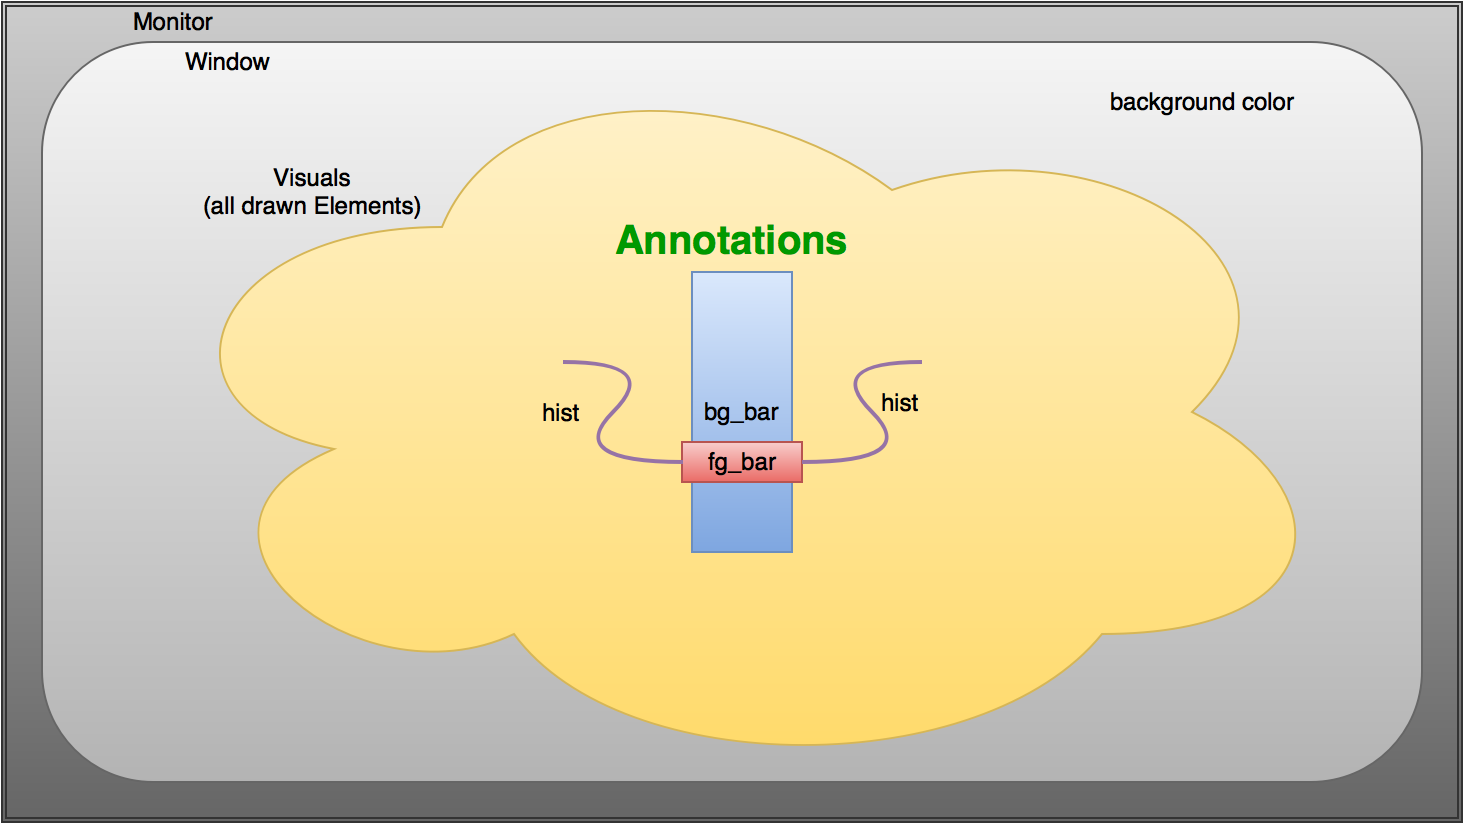
\includegraphics[width = \linewidth]{ressources/urge_graph}
\caption{Program logic of graphical objects.}
\label{fig:graph_log}
\end{figure}

\textbf{NOTE:} All visual parameters are usually set with a \emph{*.ini} file (either \textit{defaults.ini} or a run \textit{ini}-file, always in the section \verb|[visuals]|) and remain set that way over the whole runtime. However the underlying class also allows changes of all properties at runtime. In future version the option to dynamically change some of the visual elements (e.g. appearing and disappearing annotations) might be added.

All positions, height and widths (except when noted otherwise) are given in degree of the visual field. Note that size in degrees of the visual field can only be computed correctly if the monitor object is set correct. It is recommended to keep all stimuli within the central visual field, spanning at most 7\degree  in each direction.

\subsubsection{Background Parameters}

Background refers to the window background and currently has only two properties to set:
\begin{itemize}
\item \textit{col} color of the window background (see \ref{sec:color_spaces})
\item \textit{pos} list of two floats, sets the center coordinates of the stimulation, all other visual elements are placed relative to this center point, defaults to \verb|[0, 0]|
\end{itemize}

\subsubsection{bg\_bar Parameters}

\textit{bg\_bar} is the reference bar over which the indicator bar (\textit{fg\_bar}) is moved. Up on this bar refers to highest possible urge; down to no urge at all.

\textit{bg\_bar} has the following properties to be set:
\begin{itemize}
\item \verb|bg_height| positive float; height of the bar, also upper border of all other visual objects (except annotations)
\item \verb|bg_width| positive float; width of the bar
\item \verb|bg_col| color of the bar (see \ref{sec:color_spaces})
\item \verb|bg_frame_width| positive integer; width of the frame around the bar in pt (points)
\item \verb|bg_frame_col| color of the frame around the bar (see \ref{sec:color_spaces}), if no frame should be displayed either set the frame color to the bar color or set the frame width to zero
\end{itemize}

%All above values can be set with class method calls at runtime without mayor performance concerns.

\subsubsection{fg\_bar Parameters}

\textit{fg\_bar} is the indicator bar which moves over the reference bar (\textit{bg\_bar}). For correct visualization it is recommended to set width a bit larger than the width of \textit{bg\_bar}.

\textit{fg\_bar} has the following properties to be set:
\begin{itemize}
\item \verb|fg_height| numeric; height of the bar
\item \verb|fg_width| numeric; width of the bar
\item \verb|fg_col| color of the bar (see \ref{sec:color_spaces})
\item \verb|fg_frame_width| numeric; width of the frame around the bar in pt (points)
\item \verb|fg_frame_col| color of the frame around the bar  (see \ref{sec:color_spaces}), if no frame should be displayed either set the frame color to the bar color or set the frame width to zero
\item \verb|fg_opacity| float, $\in [0, 1]$; opacity controls the level of transparency of the bar (allowing the \textit{bg\_bar} object to shine trough), 1 means full opacity, 0 full transparency
\end{itemize}

%All above values can be set with class method calls at runtime without mayor performance concerns.

\textbf{Note:} To display the elements with a degree of transparency (\verb|fg_opacity| $ > 0$) efficiently and correct the system needs a graphic card with built in shaders and supports OpenGL 2.1 or higher. Most (if not all) current system fulfill those requirements.

\subsubsection{hist Parameters}

\textit{hist} objects are plots that can be on the left, the right or both sides of the central bar objects. While \textit{fg\_bar} is updated with each draw (and even between the draws), \textit{hist} is updated with it's own frequency - found under \verb|[control] hist_rate| for performance balancing. \textit{hist} objects are always anchored at the sides of the \textit{fg\_bar} object.

\textit{hist} has the following properties to be set:
\begin{itemize}
\item \verb|hist_samples| positive integer; number of samples to display, \verb|hist_samples| / \verb|[control] hist_rate| gives the duration in seconds that is displayed by \textit{hist}, can be used to treat performance issues (less samples less computation)
\item \verb|hist_width| positive float; visual width of the history for each side, note that together with \verb|fg_width| this can accumulate to a total horizontal expansion bigger than 7 \degree of the visual field.
\item \verb|hist_line_width| positive integer; width of the drawn line in pt (points)
\item \verb|hist_col| color of the hist objects (see \ref{sec:color_spaces})
\item \verb|hist_fade| boolean; indicates if the hist plots fade out at their outer borders
\item \verb|hist_side| string, either \verb|'none'|, \verb|'left'|, \verb|'right'| or \verb|'both'|; indicates on which side to draw the hist plots
\end{itemize}

%All above values can be set with class method calls at runtime, but can cause severe lags due to costly restructuring of the underlying objects. Generally \emph{hist} parameters are the most effective handles to tackle performance issues.

\textbf{Note:} As fading is done though the opacity parameter the note on opacity from \textit{fg\_bar} is also applicable. To display the elements with a degree of transparency efficiently and correct the system needs a graphic card with built in shaders and supports OpenGL 2.1 or higher. Most (if not all) current system fulfill those requirements.

\textbf{Note:} \verb|hist_fade = True| can cause a drop in performance due to different structure and rendering methods. Use with care. This should be the first parameter to check if you experience performance problems.

\subsubsection{scales Parameters}

\textit{scales} is a container object that contains all marks at the \textit{bg\_bar} - lines and text labels.

\textit{scales} has the following properties to be set:
\begin{itemize}
	\item \verb|scales_text| a list of text label strings; the empty string \verb|''| means no label is displayed
	\item \verb|scales_text_pos| a list of position marks; list length has to match the length of \verb|scales_text| or has to be 1 (meaning all text labels are set with the same position mark); position marks are: \verb|'c'| (center infront of \textit{bg\_bar}), \verb|'l'|, \verb|'r'| (left or right of \textit{bg\_bar}), \verb|'a'| or \verb|'b'| (above or below the scale line)
	\item \verb|scales_text_size| a list of text sizes;  list length has to match the length of \verb|scales_text| or has to be 1 (meaning all text labels are set with the same text size)
	\item \verb|scales_text_col| color of scale labels (see \ref{sec:color_spaces}); one color is applied to all elements
	\item \verb|scales_col| color of scale lines (see \ref{sec:color_spaces}); one color is applied to all elements
	\item \verb|scales_thickness| positive integer; thickness of scale lines in pt (points)
	\item \verb|scales_widthl| positive float; width of scale lines that can be seen left of \textit{bg\_bar}
	\item \verb|scales_widthr| positive float; width of scale lines that can be seen right of \textit{bg\_bar}
\end{itemize}

Scale ticks are distributed with equal distance over the whole bar, with the first entry placed at the lower border and the last entry placed at the top border of the \textit{bg\_bar} - if only one tick is given it is placed in the middle. Therefore given a list of three scale labels will cause scale ticks at 0\%, 50\% and 100\%. A list of 4 scale labels will cause scale ticks at 0\%, 33\%, 66\% and 100\%.

\textbf{Note:} Huge values of \verb|scales_thickness| might cause visual problem, as the upper border of the scale line might be higher than the upper border of the \textit{bg\_bar}.

\textbf{Note:} Combination of scale label position marks (such as \verb|'ra'| for right of the bar and above the line) are not possible in the current implementation, but might be in future releases. Further finer configuration methods ight also follow.

\subsubsection{annote Parameters}

An \textit{annote} is an additional text displayed somewhere on the screen.

If one wants to display $k$ annotations he has to set each \textit{annote} parameter to a list of length $k$ - each entry of this lists describes a parameter of one annotation. \textit{annote} has the following parameters to be set:
\begin{itemize}
	\item \verb|aname| list of length $k$ of unique identifier strings; not really necessary \underline{yet}, but have to be set nevertheless 
	\item \verb|atext| list of length $k$ of display strings
	\item \verb|asize| list of length $k$ of text sizes (positive integers)
	\item \verb|apos| list of length $k$ of position tupels (\verb|(x,y)|)
	\item \verb|acol| list of length $k$ of colors (see \ref{sec:color_spaces})
\end{itemize}

\textbf{Note:} In the current software logic annotation names (\verb|aname|) are not necessary. However they are now part of the software with the intention to later allow those annotation to be displayed dynamically (apperaring and disapperaing, changeing text, changing properties, \dots). This feature might be realised in a future release or be removed completely.

%%%%%%%%%%%%%%%%%%%%%%%%%%%%%%%%%%%%%%%%%%%%%%%%%%%%%%%%%%%%%%%%%%%%%%%%%%%%%%%%
\chapter{Output}

When running an experiment the software writes several output files. Here all output files will be explained.

All output files are stored within the log-folder of the experiment. This log-folder is structured as follows: it contains (technical) log files and one sub-folder for each unique subject. Those subject sub-folders contain \textit{*.info} files and corresponding data files (\textit{*.csv}) for each run performed for this one subject.

\textbf{Note:} No Output file gets overwritten! If files for a current run and subject are already present - for example due to aborting the previous run - the software will save all its output files with an appended increasing number at the end of the filename - e.g. \textit{run1.csv}, \textit{run1\_1.csv}, \textit{run1\_2.csv}, \dots It is the duty of the experimenter to later identify the log files he wants to keep/use for further analysis.

\section{Log-File}

Log-files are generated on the fly and contain some run time information (when and what of some events). Those informations are useful to find faults and errors in the software flow, but are of a very technical nature and only valuable if one is willing to delve into the source code.

The root folder of the software always contains a \textit{log.txt} file. This file contains log informations from the last experiment run and gets overwritten as soon as the next run starts. When an experiment run is finished (either regularly or by abort) this file gets copied into the log folder of the experiment as \textit{log-YYYY-MM-DD hh:mm.txt} - the end time of the experiment is appended to the file name. This time stamp allows to reconstruct which measurement was conducted when generating this log, with the help of a corresponding \textit{*.info} file in the subject log folders. Note that at first sight it might be hard to find the corresponding \textit{*.info} file - a more thorough search, in which the timestamp and the reported times in the \textit{*info} file need to be compared, could be necessary at times.

\section{Info-File}

A \textit{*.info} file is created for each run. It is located in the log folder of the subject. It contains many application informations that help to understand what the software actually did.

It starts with a section \verb|[main]|, which contains the following items: \\
\verb|experiment| (the experiment name), \verb|identifier| (subject identifier), \verb|runname| (name of the run), \verb|started| (boolean, \verb|True| if the run was started correctly), \verb|finished| (boolean, \verb|True| if the run ended without errors or aborts), \verb|status| (one of \verb|Started|, \verb|Running|, \verb|Finished|, \verb|Aborted due to Error|, \verb|Aborted by User| or plain unspecific \verb|Abort|), \verb|error_code| (\verb|None| if no error occured), \verb|end_message| (if the software reports anything before closing the run it is written there), \verb|start_time| (starting time of the run), \verb|end_time| (ending time of the run), \verb|data_file| (absolute path to the \textit{*.csv} file corresponding to this \textit{*.info} file), \verb|data_file_written| (boolean, \verb|True| if the data file was written), \verb|software| (title of the software), \verb|author| (author of the software) and \verb|version| (version of the software).

The section \verb|[experiment_configuration]| contains a copy of the main section of the file \textit{exp.ini} (see \ref{sec:expini}). The section \verb|[run_configuration]| contains a compressed copy of all \verb|[control]| and \verb|[visuals]| parameters of the run.

The section \verb|[info]| contains all of the optional informations defined in \textit{exp.ini} (see \ref{sec:expini} \nameref{sec:expini}) and their respective values that have been set in the GUI.

The section \verb|[technical_information]| holds some system informations that could be gathered without big effort. No render tests and framerate meassurements are performed. Those technical informations can be used to understand problems when running the experiment: informations about active processes, working memory, paths, versions of dependencies, input and output device information, \dots If a render test is wished for it has to be performed either from within the PsychoPy GUI (Tools $\rightarrow$ Benchmark Wizard) or by calling the function \verb|psychopy.info.RunTimeInfo| manually.

\textbf{Note:} In future versions this recording of technical informations might change, since it still takes some time before starting a run and performing it once might be enough for most purposes.

\section{Data-File}

A \textit{*.csv} file is created for each run. It is located in the log folder of the subject. It contains a table with at least three columns and as much rows as urge-sample-points. The first column contains the reported urge at the sampling time-point, the second column contains the absolute sampling time-point relative to experiment onset and the third column contains latencies - the difference of absolute sampling time-point and the theoretical sampling time-point (if timing and sampling with the computer was perfect). This third column - latency - is a good indicator of problems at runtime. If latencies are close to the theoretical sampling interval ($1 / $\verb|sampling_rate|) or have a very high variability it can be read as an inidcator of runtime problems, which could make one worry about data quality. A close look at the computer running the experiment and the configuration parameters could help identify and solve runtime problems. 

After the first three columns a number of additional columns is possible, depending on the configuration of the experiment. For each additional button to log one column is created. It contains zeros where no button press occurred and ones where the specific button was pressed. Those additional columns are appended in the order of the \verb|log_buttons| entry of \textit{exp.ini} - \verb|log_buttons = ['y', 'x', 'c']| means that the fourth column represents presses of button \verb|'y'|, the fifth of button \verb|'x'| and the sixth of button \verb|'c'|.

The table always contains enough rows to record the complete run. If a run gets aborted early the rows that have not yet been set are filled with \verb|NA| (stands for: Not A Number).

The data file gets written to the hard-drive as soon as the run ends - either regularly, after abort or after an software error. If the computer crashes while running an experiment run, data recorded till the time-point of the crash is lost, since it has not been written prior to the crash.

Those \textit{*.csv} files can be opened easily with any modern table calculation program - e.g. Microsoft Excel, LibreOffice Calc, \dots Data from those files can also be imported into a number of analysis programs, such as MATLAB, SPSS, SAS, R, \dots Those files are very clean CSV files - no strings, decimal point, separator is \verb|,|, line breaks are row breaks, all lines ahve the same length, no headers - so reading and importing those files should not pose any problem for most software. If such a reading problem occures one has to work the parameters of the reading program when opening those files.
\end{document}